\chapter{Технологический раздел}

\section{Модели}

Веб-приложения Django получают доступ и управляют данными через объекты Python, называемые моделями.
Модели определяют структуру хранимых данных, включая типы полей и, возможно, их максимальный размер, значения по умолчанию, параметры списка выбора, текст справки для документации, текст меток для форм и т.~д.

В листингах \ref{lst:Article}–\ref{lst:Vote} представлены все модели, соответствующие структуре базы данных, за исключением стандартной модели \code{django.contrib.auth.models.User}.

\lstinputlisting[
	caption={Модель статьи},
	label={lst:Article},
	language=Python,
	linerange={11-19}
]{../myblog/models/article.py}

\lstinputlisting[
	caption={Модель комментария},
	label={lst:Comment},
	language=Python,
	linerange={10-17}
]{../myblog/models/comment.py}

\lstinputlisting[
	caption={Модель тэга},
	label={lst:Tag},
	language=Python,
	linerange={7-9}
]{../myblog/models/tag.py}

\lstinputlisting[
	caption={Модель голоса},
	label={lst:Vote},
	language=Python,
	linerange={7-17}
]{../myblog/models/vote.py}

В листинге \ref{lst:sqlmigrate} (приложении А, стр. \pageref{chp:attachment-a}) представлен SQL запрос на создание базы данных, сгенерированный фреймворком Django на основе существующих моделей ()получено командой \code{python3 manage.py sqlmigrate myblog 0001}, приведено к удобочитаемому виду).

\section{Менеджеры}

Наиболее важным атрибутом модели является Manager.
Это интерфейс, посредством которого осуществляются операции запросов к базе данных от моделей Django и используются для извлечения экземпляров из базы данных.
Если пользовательский Manager не определен, по умолчанию используется имя objects \cite{django-mozilla}.

В листингах \ref{lst:OrderedQuerySet} и \ref{lst:ArticleQuerySet} реализованы менеджеры, используемые моделями.

\lstinputlisting[
	caption={Менеджер с функциями упорядочивания},
	label={lst:OrderedQuerySet},
	language=Python,
	linerange={4-15}
]{../myblog/managers/ordered.py}

\lstinputlisting[
	caption={Менеджер для работы со списком статей},
	label={lst:ArticleQuerySet},
	language=Python,
	linerange={4-12}
]{../myblog/managers/article.py}

\section{Представления}

Django использует представления для инкапсуляции логики обработки запроса и ответа на этот запрос.

В листинге \ref{lst:VoteView} показано представление голосов \code{VoteView}, обрабатывающее POST запрос на изменение рейтинга статьи или комментария.
Изменения заносятся в таблицу голосов Vote (\ref{tbl:myblog_vote}), рейтинг объекта (статьи или комментария) обновляется непосредственно в записи соответствующей таблицы (атрибут \code{rating}).

\lstinputlisting[
	caption={Представление голосов},
	label={lst:VoteView},
	language=Python,
	linerange={10-42}
]{../myblog/views/vote.py}

Остальные представления можно найти в приложении Б (стр. \pageref{chp:attachment-b}).

\section{URL}

Для разработки URL-адресов приложения в Django необходимо создать модуль Python, называемый URLconf.
URLconf — это набор шаблонов, которые Django попробует сравнить с полученным URL, чтобы выбрать правильный метод для представления (view).
Django сопоставляет URL-адреса, используя регулярные выражения.
Регулярные выражения имеют множество правил, которые формируют поисковый шаблон.
В листинге \ref{lst:urlpatterns} представлен список URL-шаблонов в проекте.

\lstinputlisting[
	caption={Список URL-шаблонов},
	label={lst:urlpatterns},
	language=Python,
	linerange={10-37}
]{../myblog/urls.py}

\section{Frontend-разработка}

Пользовательский интерфейс при разработке web-приложения представляет из себя полноценную вёрстку проекта.

Bootstrap — это инструментарий с открытым исходным кодом для разработки web-приложений с помощью HTML, CSS и JS.
Включает в себя HTML- и CSS-шаблоны оформления для типографики, веб-форм, кнопок, меток, блоков навигации и прочих компонентов веб-интерфейса, включая JavaScript-расширения \cite{bootstrap}.
С помощью него настроен дизайн сайта.

В Django есть удобный способ динамического генерирования HTML, основанный на шаблонах.
Шаблон содержит статические части желаемого вывода HTML, а также некоторый специальный синтаксис, описывающий, как будет вставляться динамический контент.
Фреймворк Django поставляет встроенный бэкэнд для своей системы шаблонов, называемой языком шаблонов Django (DTL) \cite{django}.

В листинге \ref{lst:template-article} для представлен шаблона страницы статьи.
Остальные шаблоны можно найти в приложении В (стр. \pageref{chp:attachment-c}).

\lstinputlisting[
	caption={Шаблон страницы статьи},
	label={lst:template-article},
	language=HTML
]{../myblog/templates/myblog/article.html}

В листинге \ref{lst:js} представлен скрипт, добавляющий кнопкам голосов (upvote, downvote) интерактивность.
Формируется POST запрос с захватом CSRF-токена, обработчик которого был представлен в листинге \ref{lst:VoteView}.

\lstinputlisting[
	caption={main.js},
	label={lst:js},
	language=JavaScript
]{../myblog/static/myblog/js/main.js}

\section{Интерфейс приложения}

На рисунках \ref{img:runtime-feed-and-article}--\ref{img:runtime-article-update} продемонстрированы основные экраны приложения.

\begin{figure}[H]
	\centering
	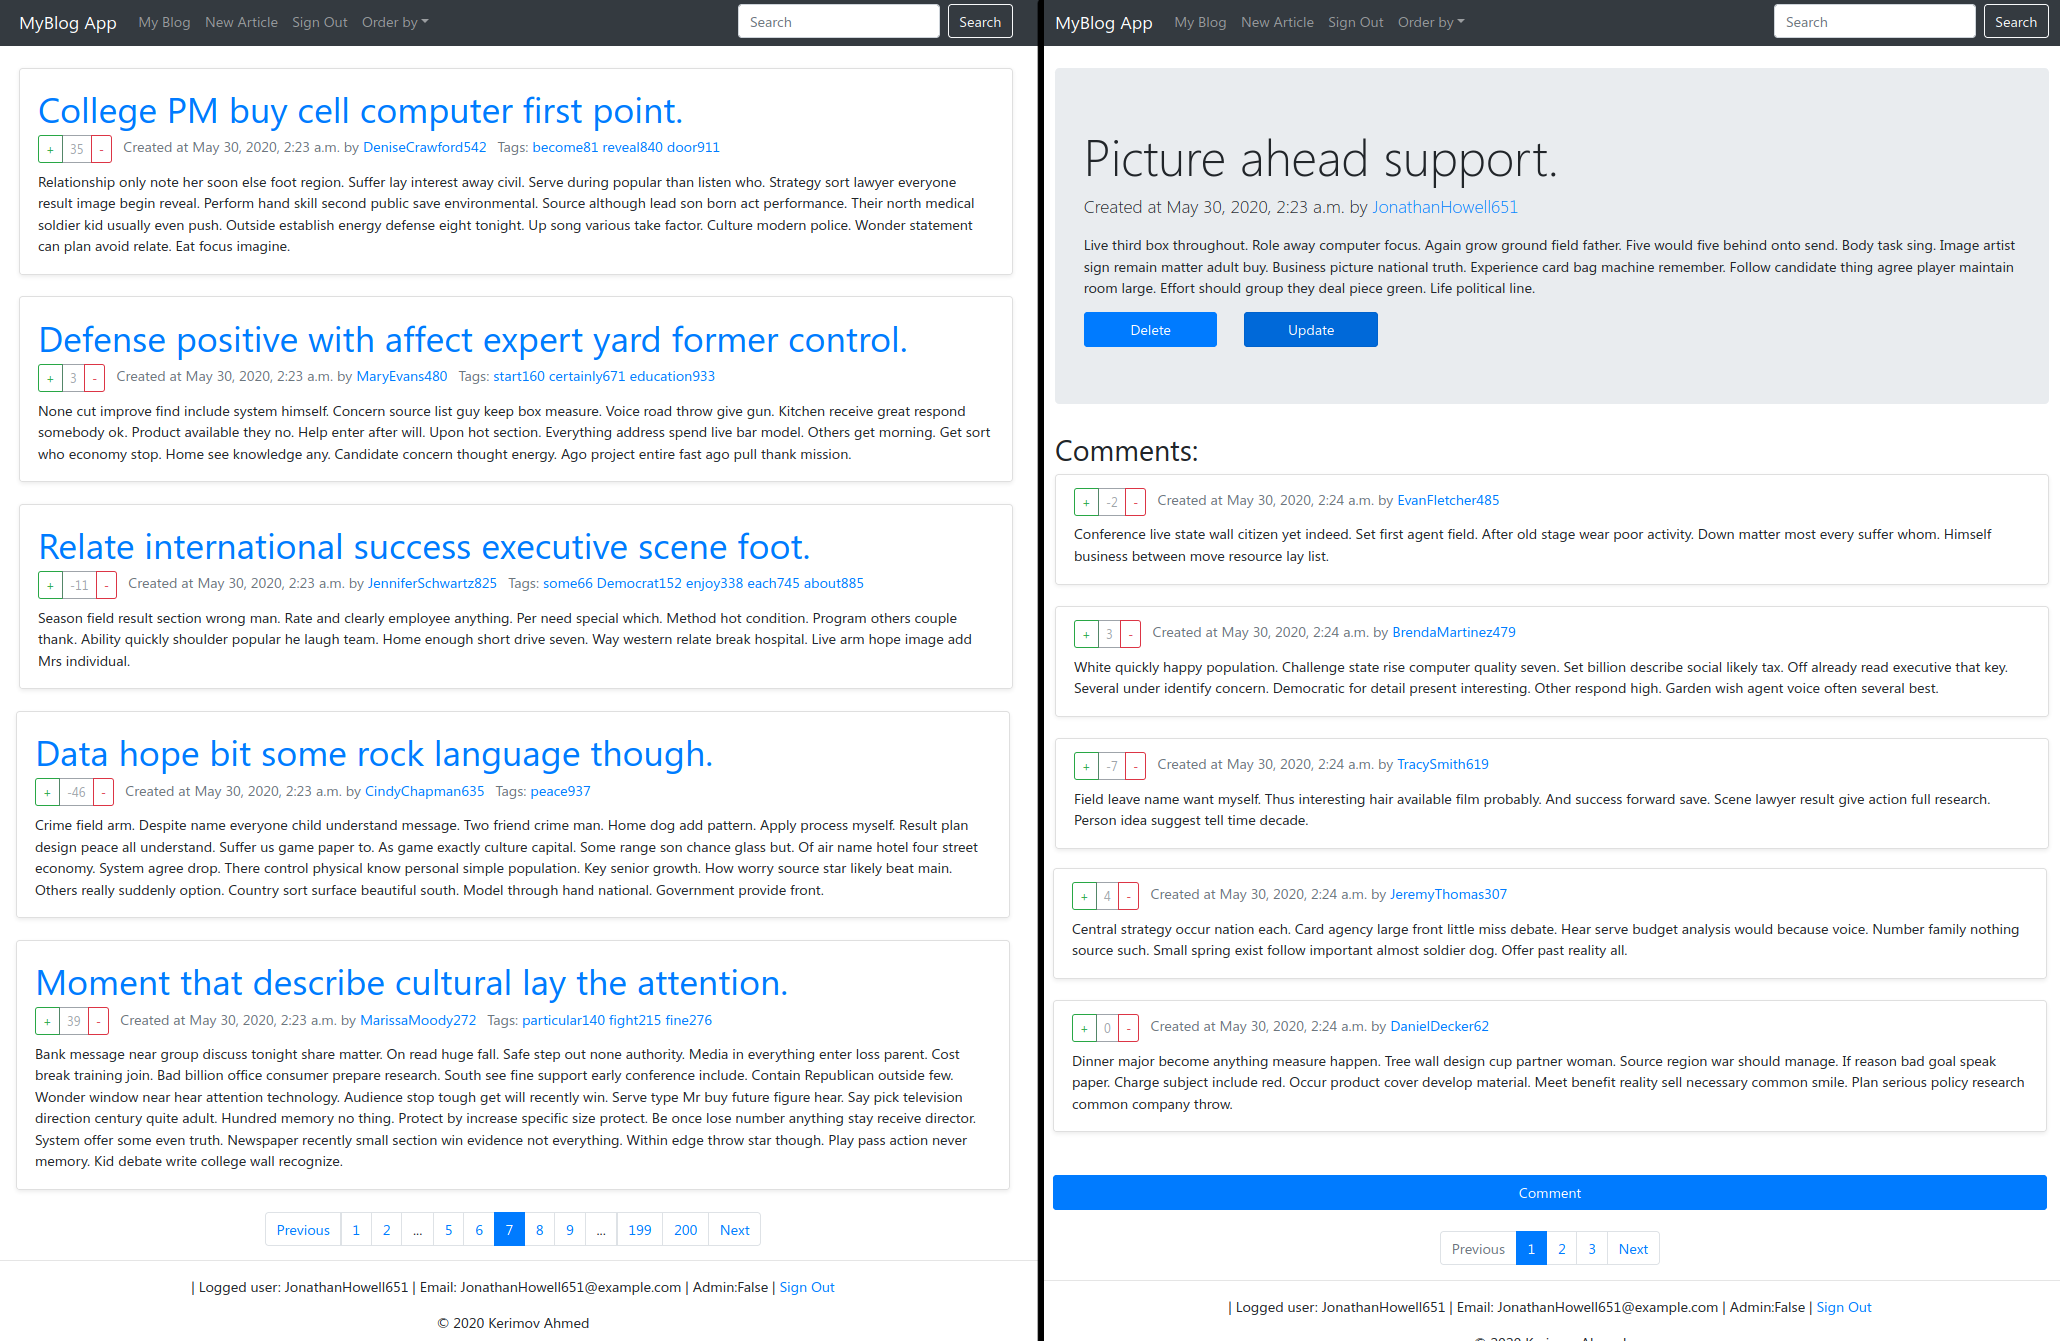
\includegraphics[width=\linewidth]{inc/img/runtime-feed-and-article}
	\caption{Страница ленты статей (слева) и страница статьи (справа)}
	\label{img:runtime-feed-and-article}
\end{figure}

\begin{figure}[H]
	\centering
	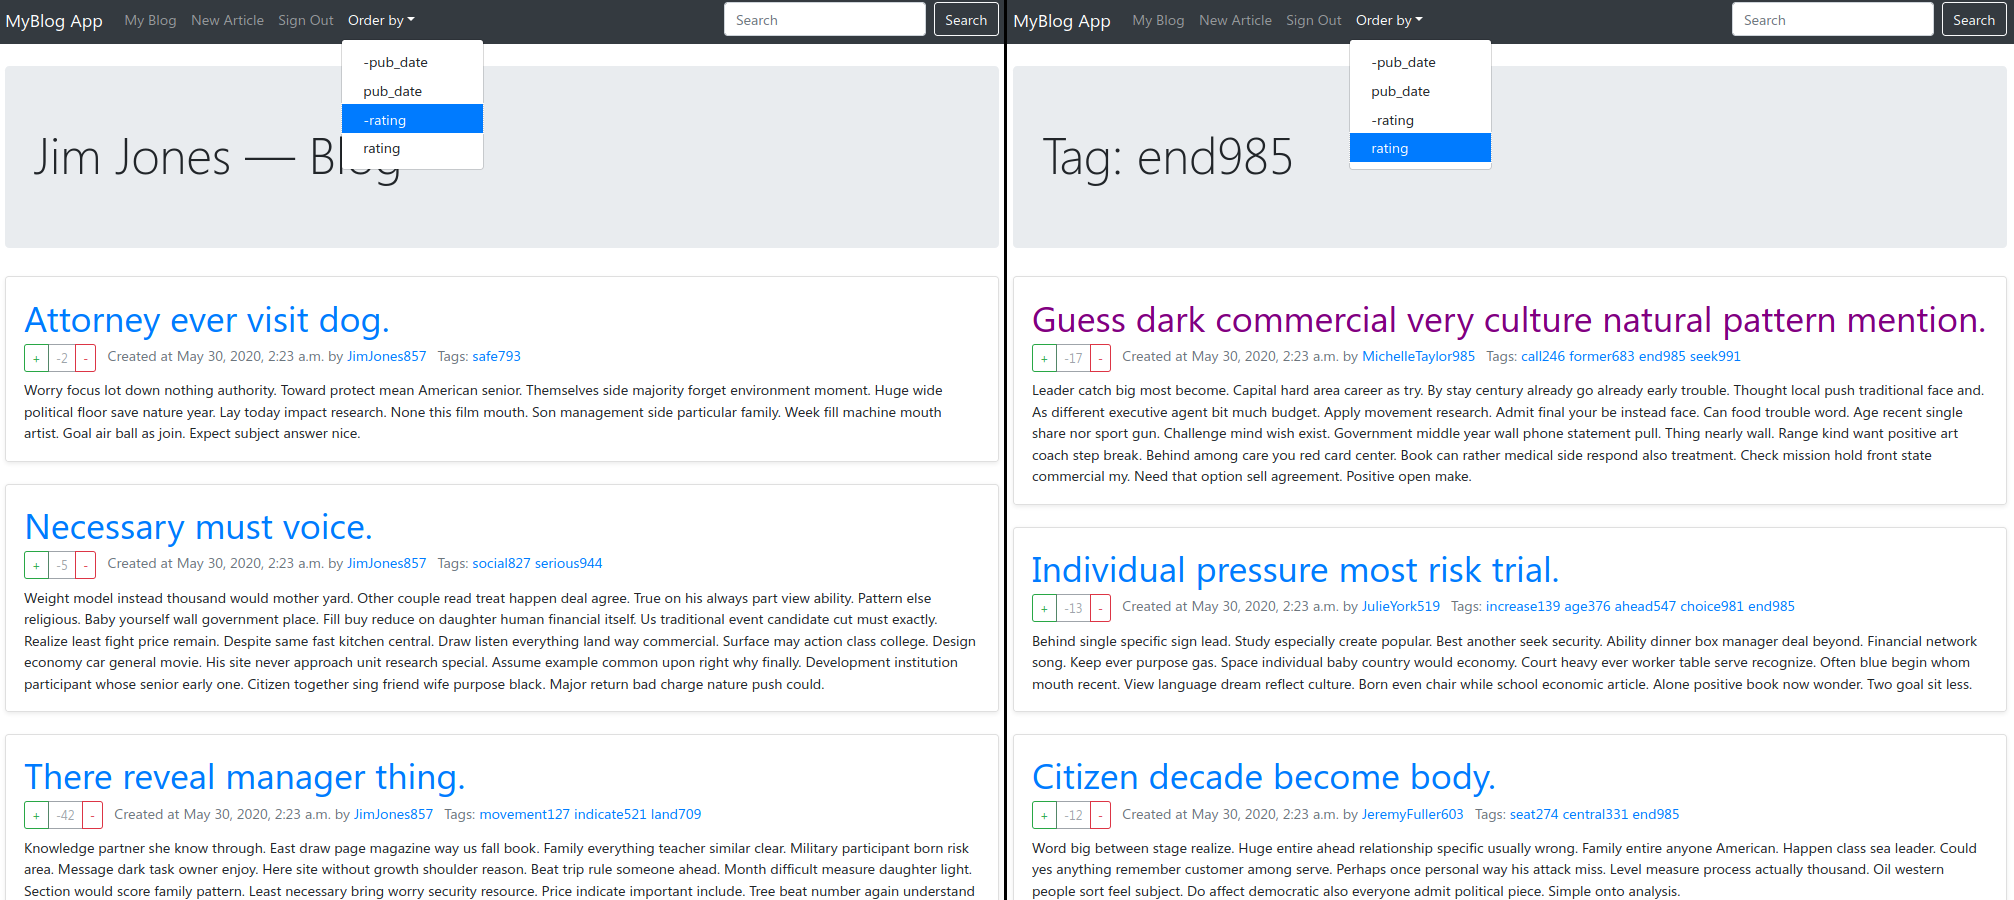
\includegraphics[width=\linewidth]{inc/img/runtime-blog-tag}
	\caption{Страница блога (слева) и фильтрация по тэгу (справа)}
	\label{img:runtime-blog-tag}
\end{figure}

\begin{figure}[H]
	\centering
	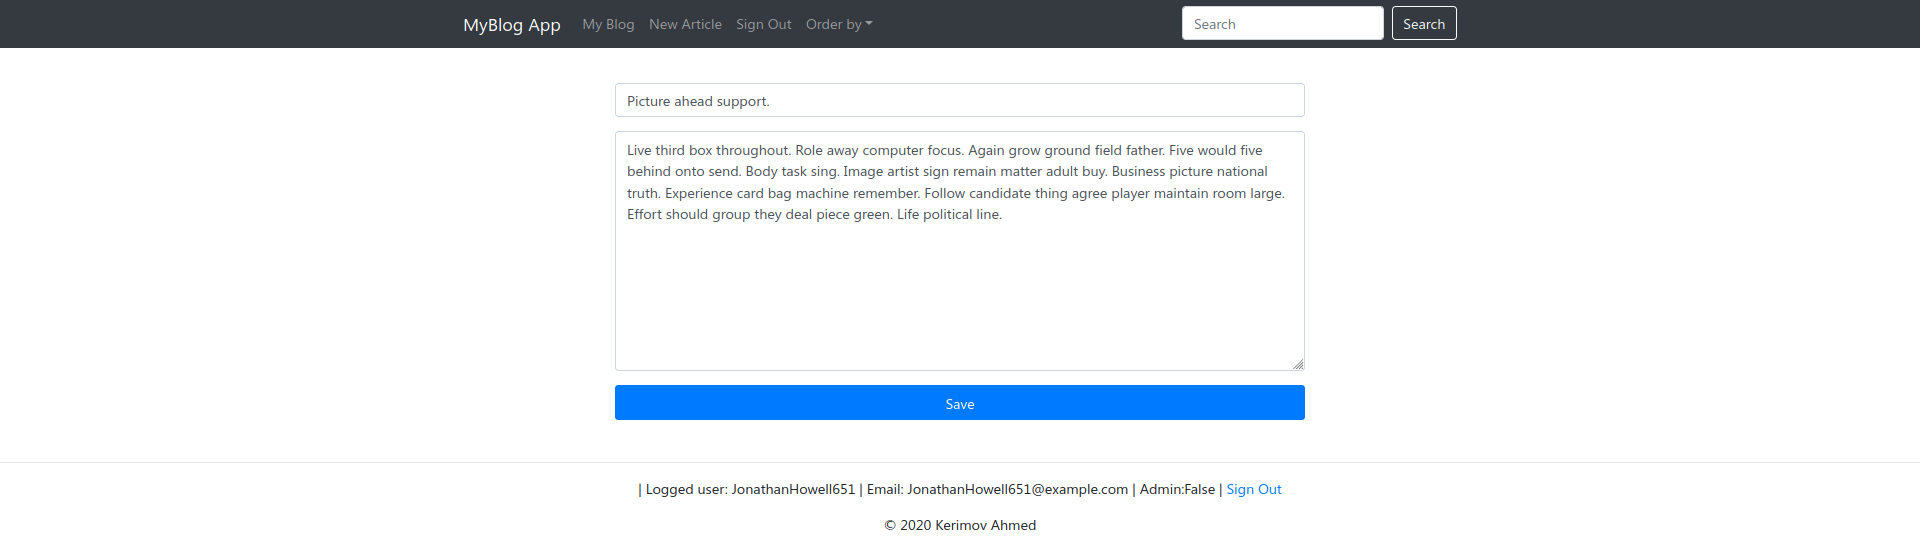
\includegraphics[width=\linewidth]{inc/img/runtime-article-update}
	\caption{Страница обновления статьи}
	\label{img:runtime-article-update}
\end{figure}

\section{Заполнение базы данных}

Первое, о чем стоит задуматься при создании базы данных — это её наполнение.
В проекте достаточно большое количество таблиц и сущностей, поэтому задача ее наполнения – важнейший аспект работы, так как на реальных пользователях проверить работу сейчас невозможно.
Был написан скрипт на языке Python, который создает сущности в таком порядке: пользователи, тэги, статьи, комментарии и голоса.
Такой порядок важен, т.~к. без тэгов и пользователей невозможно создать статьи, без статьей невозможно создать комментарии и т.~д.
Количество сгенерированных записей можно редактировать параметрами командной строки.
Листинг программы генерации фейковых данных представлен в приложении С (стр. \pageref{chp:attachment-d}).

\section*{Вывод}

С помощью выбранных средств разработки и ранее спроектированной базы данных была создана платформа для ведения онлайн-дневников (блогов), а также написан скрипт генерации фейковых данных для заполнения БД.
